\section{Exponential Distribution}

\subsection{Standard Exponential Distribution}

The PDF of the exponential distribution is

\begin{equation}
	p(x| \lambda) = \lambda \exp(-\lambda x)
	\label{eq:exponential_pdf}
\end{equation}

which can be written as

\begin{equation}
	p(x|\lambda) = \exp\left[-\lambda x + \log\lambda\right]
	\label{eq:exponential_exp_family}
\end{equation}

with $T=x$, $\eta = -\lambda$ and $A(\lambda) = -\log\lambda$

\subsubsection{Laplace Approximation of the Exponential Distribution}

\begin{align*}
\text{log-pdf: } &\left( \log \lambda - \lambda x\right) \\
\text{1st derivative: }& - \lambda \\
\text{2nd derivative: }& 0
\end{align*}
The Laplace Approximation is not defined since the second derivative is not positive. 

\subsection{Log-transformed Exponential Distribution}

We choose $g(x) = \log(x)$, and thereby $g^{-1}(x) = \exp(x)$. It follows that the new pdf is 

\begin{align}
	f(x|\lambda) &= \lambda \exp(-\lambda \exp(x)) \cdot \exp(x) \\ \nonumber
	&= \lambda \exp(-\lambda \exp(x) + x)
\end{align}

which can be written as 


\begin{equation}
	p(x|\lambda) = \exp\left[-\lambda \exp(x) + x + \log\lambda\right]
	\label{eq:exponential_exp_family_trans}
\end{equation}

with $T= x, \exp(x)$, $\eta = 1, -\lambda$ and $A(\lambda)=\log\lambda$

\subsubsection{Laplace Approximation of the log-transformed Exponential Distribution}

\begin{align*}
\text{log-pdf: } & -\lambda \exp(x) + x + \log\lambda \\
\text{1st derivative: }& \lambda -\exp(x) + 1 \\
\text{mode: } & x = \log(1/\lambda) \\
\text{2nd derivative: }& \lambda -\exp(x)\\
\text{insert mode: }& -\lambda\exp(1/\lambda) = -1\\
\text{invert: }&\sigma^2 = 1
\end{align*}

Therefore the Laplace approximation in the transformed basis is given by $\mathcal{N}(x, \log(1/\lambda), 1)$. 

\subsection{The Bridge}

We have already found $\mu$ and $\sigma$. The inverse transformation is easily found through the mode $x = \log(1/\lambda) \Leftrightarrow \lambda = 1/\exp(x)$. In summary:

\begin{align}
	\mu &= \log(1/\lambda) \\
	\sigma &= 1 \\
	\lambda &= 1/\exp(x)
\end{align}

\begin{figure}
	\centering
	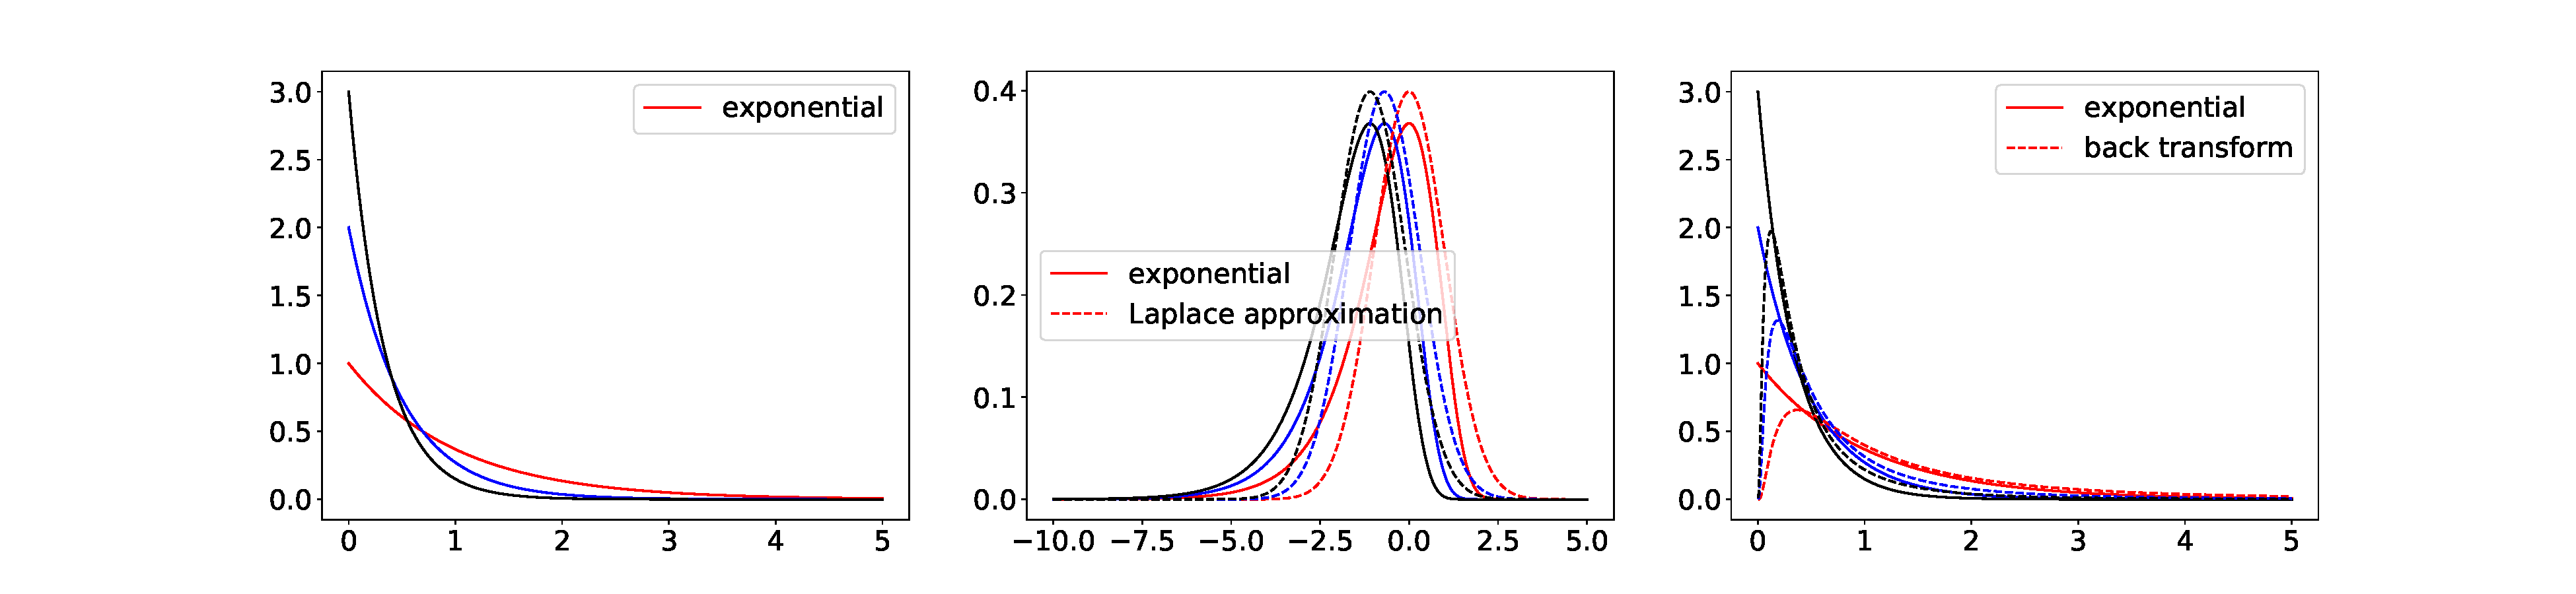
\includegraphics[width=\textwidth]{figures/exponential_playground.pdf}
	\caption{exponential comparison}
	\label{fig:exponential_comparison}
\end{figure}